\chapter{Risultati}

In questo capitolo verranno presentati i principali risultati ottenuti dalle simulazioni eseguite. Ne sono state effettuate diverse, con varie configurazioni. Verranno valutati l'algoritmo di placement al variare di specifici parametri ed, eventualmente, il soddisfacimento delle richieste con e senza failure control.

\section{Simulazioni con Variazione di Singoli Parametri}

\subsection{Simulazione con Variazione della Privacy}

In questo scenario l'algoritmo di placement è stato eseguito undici volte. Ad ogni esecuzione viene incrementato il valore di privacy di 10 unità, partendo da 0 fino a 100. Si ricorda che il valore di privacy indica il livello massimo, nell'architettura di riferimento, in cui un servizio può essere allocato. Il parametro che varia è in particolare \texttt{PRIVACY\_ASSIGNMENT}. Questo parametro indica la percentuale di servizi a cui il valore di privacy viene assegnato.

Come si può vedere dal grafico in Figura \ref{fig:privacy_placement_success}, l'algoritmo di placement ha un successo accettabile fino ad un valore di privacy pari a 60, con un successo del posizionamento della applicazioni pari al $60\%$. Da questo valore in poi il successo cala drasticamente.

\begin{figure}[!ht]
  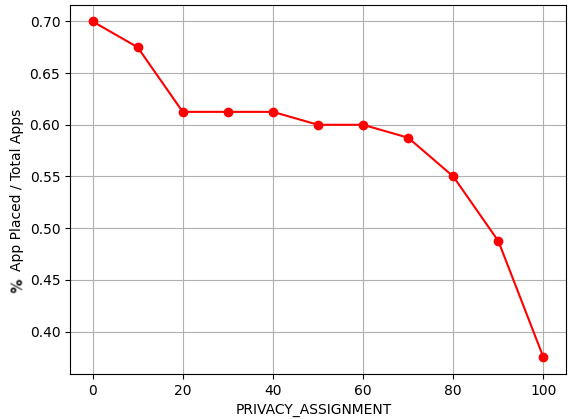
\includegraphics[width=10cm]{images/privacy_placement_success}
  \centering
  \caption{Successo dell'algoritmo di placement al variare del parametro \texttt{PRIVACY\_ASSIGNMENT}.}
  \label{fig:privacy_placement_success}
\end{figure}

Ciò che maggiormente si evince dal grafico in Figura \ref{fig:privacy_placement_per_level} è che il livello Cloud viene utilizzato solo per l'1.5\%. Si ricorda che il compito del Cloud è quello di fungere da nodo utile per i servizi che non hanno trovato un nodo Fog disponibile in fase di placement. Il valore di privacy non può quindi crescere troppo.

\begin{figure}[!ht]
  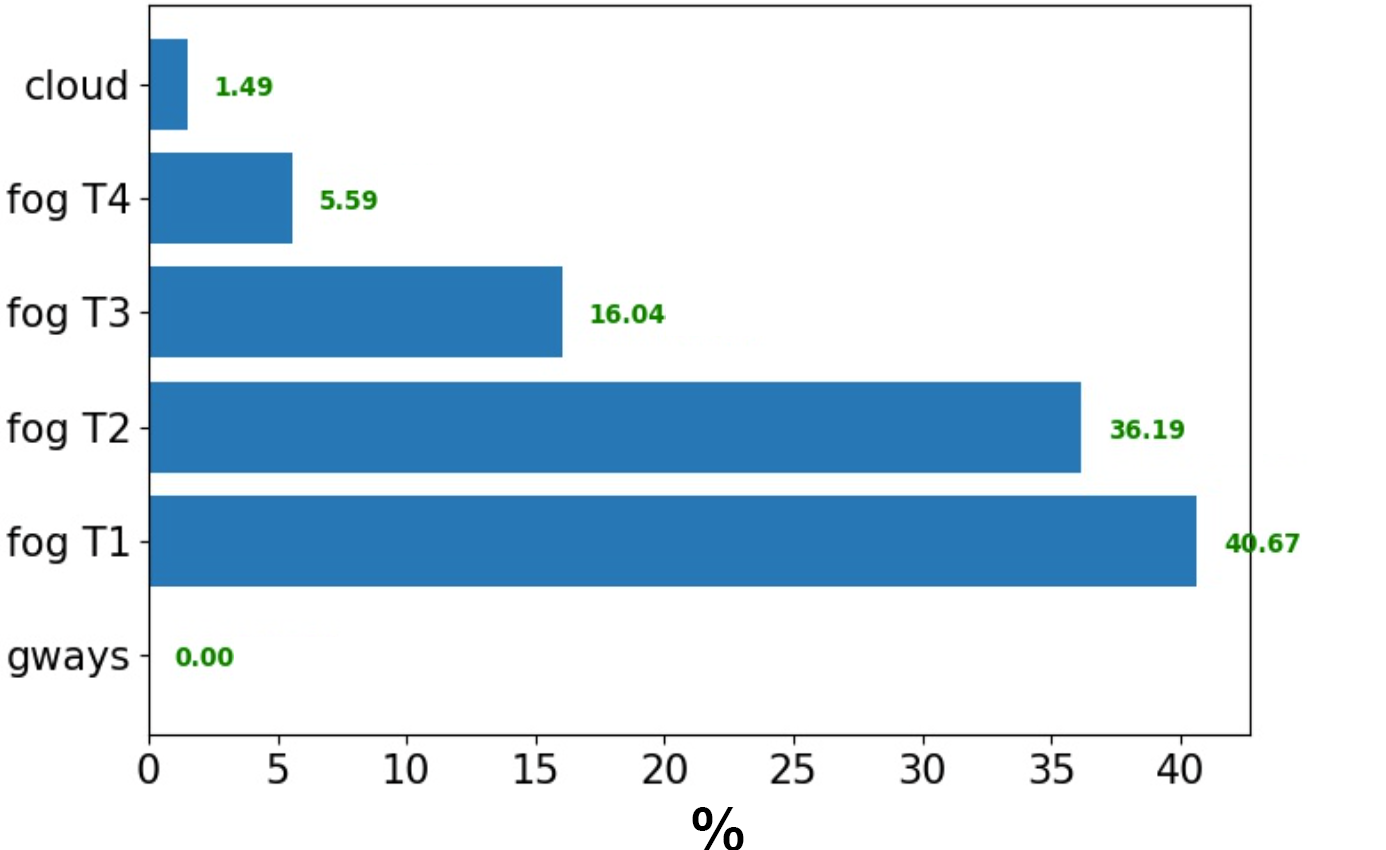
\includegraphics[width=10cm]{images/privacy_placement_per_level}
  \centering
  \caption{Percentuale di servizi allocati in ogni livello.}
  \label{fig:privacy_placement_per_level}
\end{figure}

È stata inoltre valutato, con questo valore di privacy, il soddisfacimento delle richieste con e senza failure control. Questo risultato è mostrato nel grafico in Figura \ref{fig:privacy70_simulation_result}.

\begin{figure}[!ht]
  \includegraphics[width=14cm]{images/privacy70_simulation_result}
  \centering
  \caption{Numero di richieste soddisfatte durante la simulazione, con e senza failure control.}
  \label{fig:privacy70_simulation_result}
\end{figure}

\subsection{Simulazione con Variazione delle Risorse Richieste dai Servizi}

In questo scenario l'algoritmo di placement è stato eseguito dieci volte. Ad ogni esecuzione viene incrementato il valore corrispondente alle risorse richieste dai servizi. Il parametro in questione è \texttt{FUNC\_SERVICE\_RESOURCES}. Il successo dell'algoritmo di placement al variare di tale parametro è mostrato nel grafico in Figura \ref{fig:resources_placement_success}. Il risultato principale che si evince dal grafico è la velocità con il quale decresce la percentuale di applicazioni correttamente allocate. Infatti aumentando, anche di poco, il numero di risorse richieste poche applicazioni vengono allocate.

\begin{figure}[!ht]
  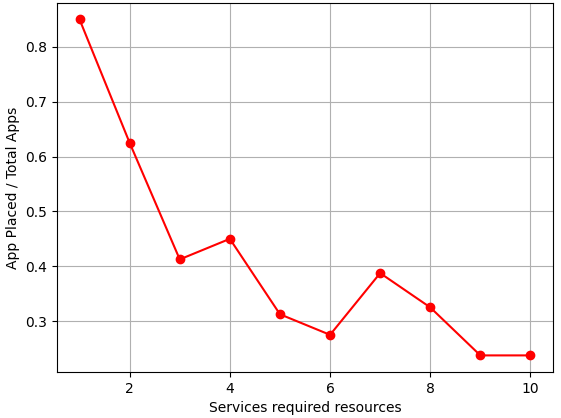
\includegraphics[width=10cm]{images/resources_placement_success}
  \centering
  \caption{Successo dell'algoritmo di placement al variare del parametro \texttt{FUNC\_SERVICE\_RESOURCES}.}
  \label{fig:resources_placement_success}
\end{figure}

È stata eseguita una simulazione con \texttt{FUNC\_SERVICE\_RESOURCES} pari a \texttt{random.randint(7, 10)}. Le risorse allocate per livello sono mostrate nel grafico in Figura \ref{fig:resources_placement_per_level}. In questo caso come si evince dal grafico in Figura \ref{fig:resources_placement_success}, sono state allocate correttamente circa il 40\% delle applicazioni.

\begin{figure}[!ht]
  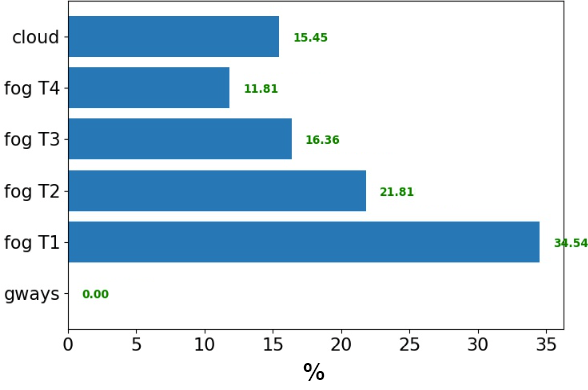
\includegraphics[width=10cm]{images/resources_placement_per_level}
  \centering
  \caption{Percentuale di servizi allocati in ogni livello}
  \label{fig:resources_placement_per_level}
\end{figure}

\subsection{Simulazione con Variazione del Fattore di Riduzione dei Nodi nei Livelli Superiori}

In questo scenario l'algoritmo di placement è stato eseguito 21 volte, facendo variare il parametro \texttt{REDUCTION\_FACTOR\_2}, incrementandolo di 0.1 ad ogni iterazione. Questo parametro regola la riduzione del numero di nodi Fog da un livello a quello successivo. Quando \texttt{REDUCTION\_FACTOR\_2} è pari a 1 il numero di nodi Fog non varia, viceversa quando questo valore è pari a 3 il numero di nodi Fog ad un determinato livello $n$ sarà pari ad $1/3$ del numero di nodi del livello $n-1$.

I risultati dell'esecuzione consecutiva dell'algoritmo di placement è mostrato nel grafico in Figura \ref{fig:YAFS_classes}

\begin{figure}[!ht]
  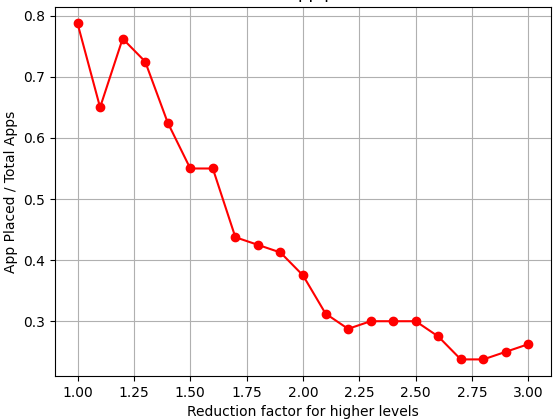
\includegraphics[width=10cm]{images/nodes_number_placement_success}
  \centering
  \caption{Successo dell'algoritmo di placement al variare del parametro \texttt{REDUCTION\_FACTOR\_2}.}
  \label{fig:nodes_number_placement_success}
\end{figure}

Ciò che si evince dal grafico è che, salvo alcune oscillazioni, la tendenza è fortemente decrescente. Infatti oltre al valore 1.5 il successo dell'algoritmo di placement cala drasticamente. 

Per evidenziare quanto detto vengono riportati in Figura \ref{fig:reduction_factor_placement_comparison} i grafici raffiguranti la percentuale di servizi correttamente allocati per ogni livello. A destra viene mostrato il grafico ottenuto impostando il valore di \texttt{REDUCTION\_FACTOR\_2} pari a 1, a sinistra pari a 3. 

Ciò che si evince è che l'algoritmo di placement, grazie alla sua natura greedy, ha allocato in entrambi i casi la percentuale maggiore di servizi nel primo livello. Nel primo caso però molti servizi sono stati allocati nei livelli superiori, con una percentuale che differisce di poche unità, mentre nei livelli superiori, dato il numero molto più basso di nodi disponibili, dove cala drasticamente il successo di placement, cala conseguentemente anche il numero di servizi per livello.

\begin{figure}[!ht]
  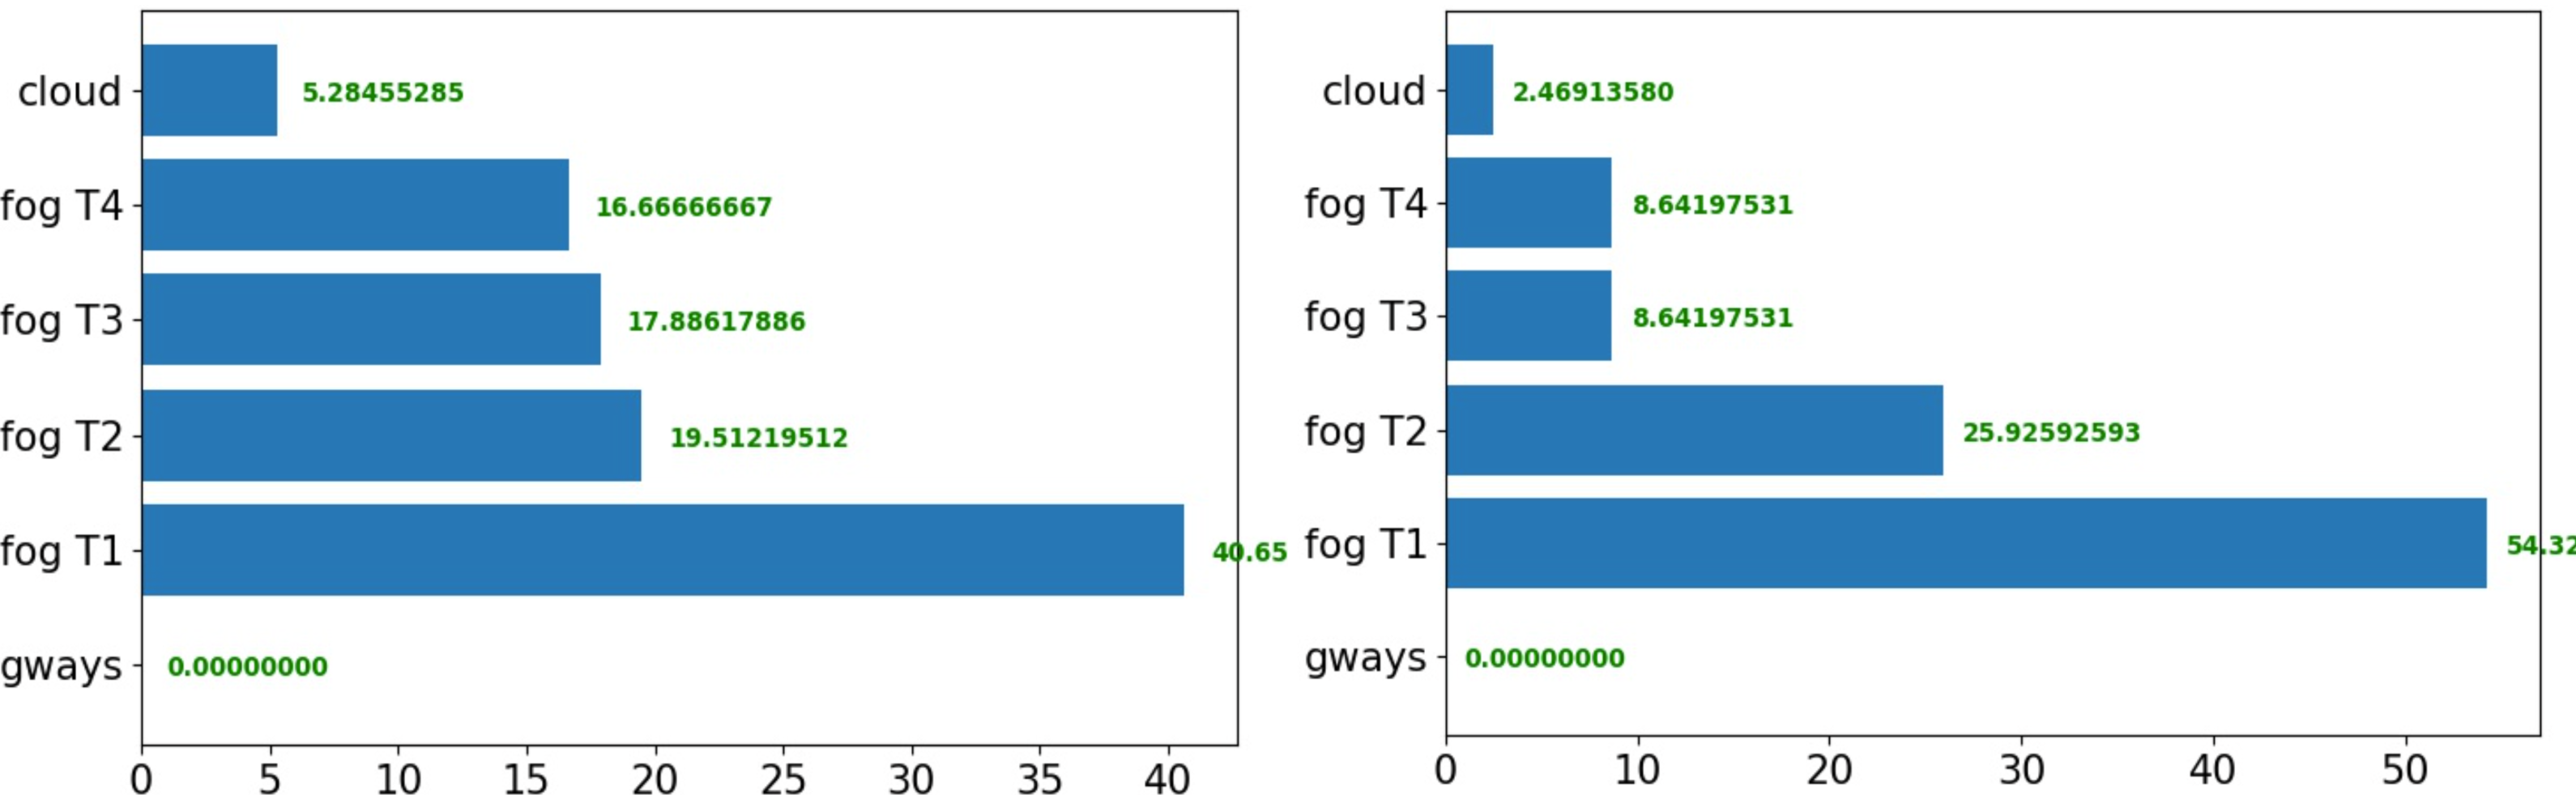
\includegraphics[width=14cm]{images/reduction_factor_placement_comparison}
  \centering
  \caption{Percentuale di servizi correttamente allocati in ogni livello. A sinistra con \texttt{REDUCTION\_FACTOR\_2} pari a 1, a destra con \texttt{REDUCTION\_FACTOR\_2} pari a 3.}
  \label{fig:reduction_factor_placement_comparison}
\end{figure}

\subsection{Simulazione con Variazione del Numero di Connessioni dai Livelli Inferiori ai Livelli Superiori}

In questo scenario è stato eseguito 20 volte l'algoritmo di placement facendo variare il numero di connessioni di ogni nodo dai livelli inferiori ai livelli superiori. In particolare sono stati fatti variare i variare i parametri \texttt{MIN\_CONN\_TO\_UPPER\_LEVELS} e \texttt{MAX\_CONN\_TO\_UPPER\_LEVELS} da 10 e 20, rispettivamente, a 200 e 210.

Il successo del placement al variare di tali parametri è mostrato nel grafico in Figura \ref{fig:minmax_conn_to_upper}

\begin{figure}[!ht]
  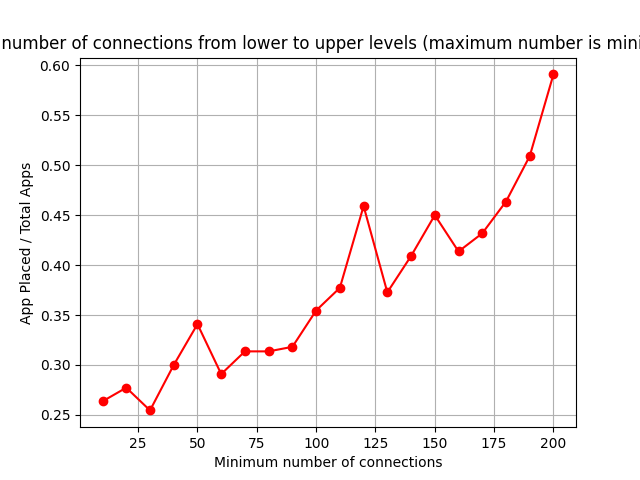
\includegraphics[width=10cm]{images/minmax_conn_to_upper}
  \centering
  \caption{Successo dell'algoritmo di placement al variare del parametro \texttt{MIN\_CONN\_TO\_UPPER\_LEVELS}.}
  \label{fig:minmax_conn_to_upper}
\end{figure}

Dal grafico si evince che all'aumentare del valore relativo al numero minimo di coonnesioni verso i livelli più alti aumenta il successo dell'algoritmo di placement. Il fattore di maggiore rilevanza è rappresentato dal fatto che all'aumentare delle connessioni verso i livelli alti vengono garantite un numero sempre maggiore di strade per poter allocare servizi ai nodi più alti. Per sottolineare quanto detto, sono stati eseguite due simulazioni, una con \texttt{MIN\_CONN\_TO\_UPPER\_LEVELS = 10} e \texttt{MAX\_CONN\_TO\_UPPER\_LEVELS = 20}, l'altra con \texttt{MIN\_CONN\_TO\_UPPER\_LEVELS = 200} e \texttt{MAX\_CONN\_TO\_UPPER\_LEVELS = 210}. Per ognuna delle due sono stati prodotti i grafici, mostrati in Figura \ref{fig:min_conn_to_upper_levels_comparison}, relativi alla percentuale di servizi che vengono allocati nei vari livelli.

\begin{figure}[!ht]
  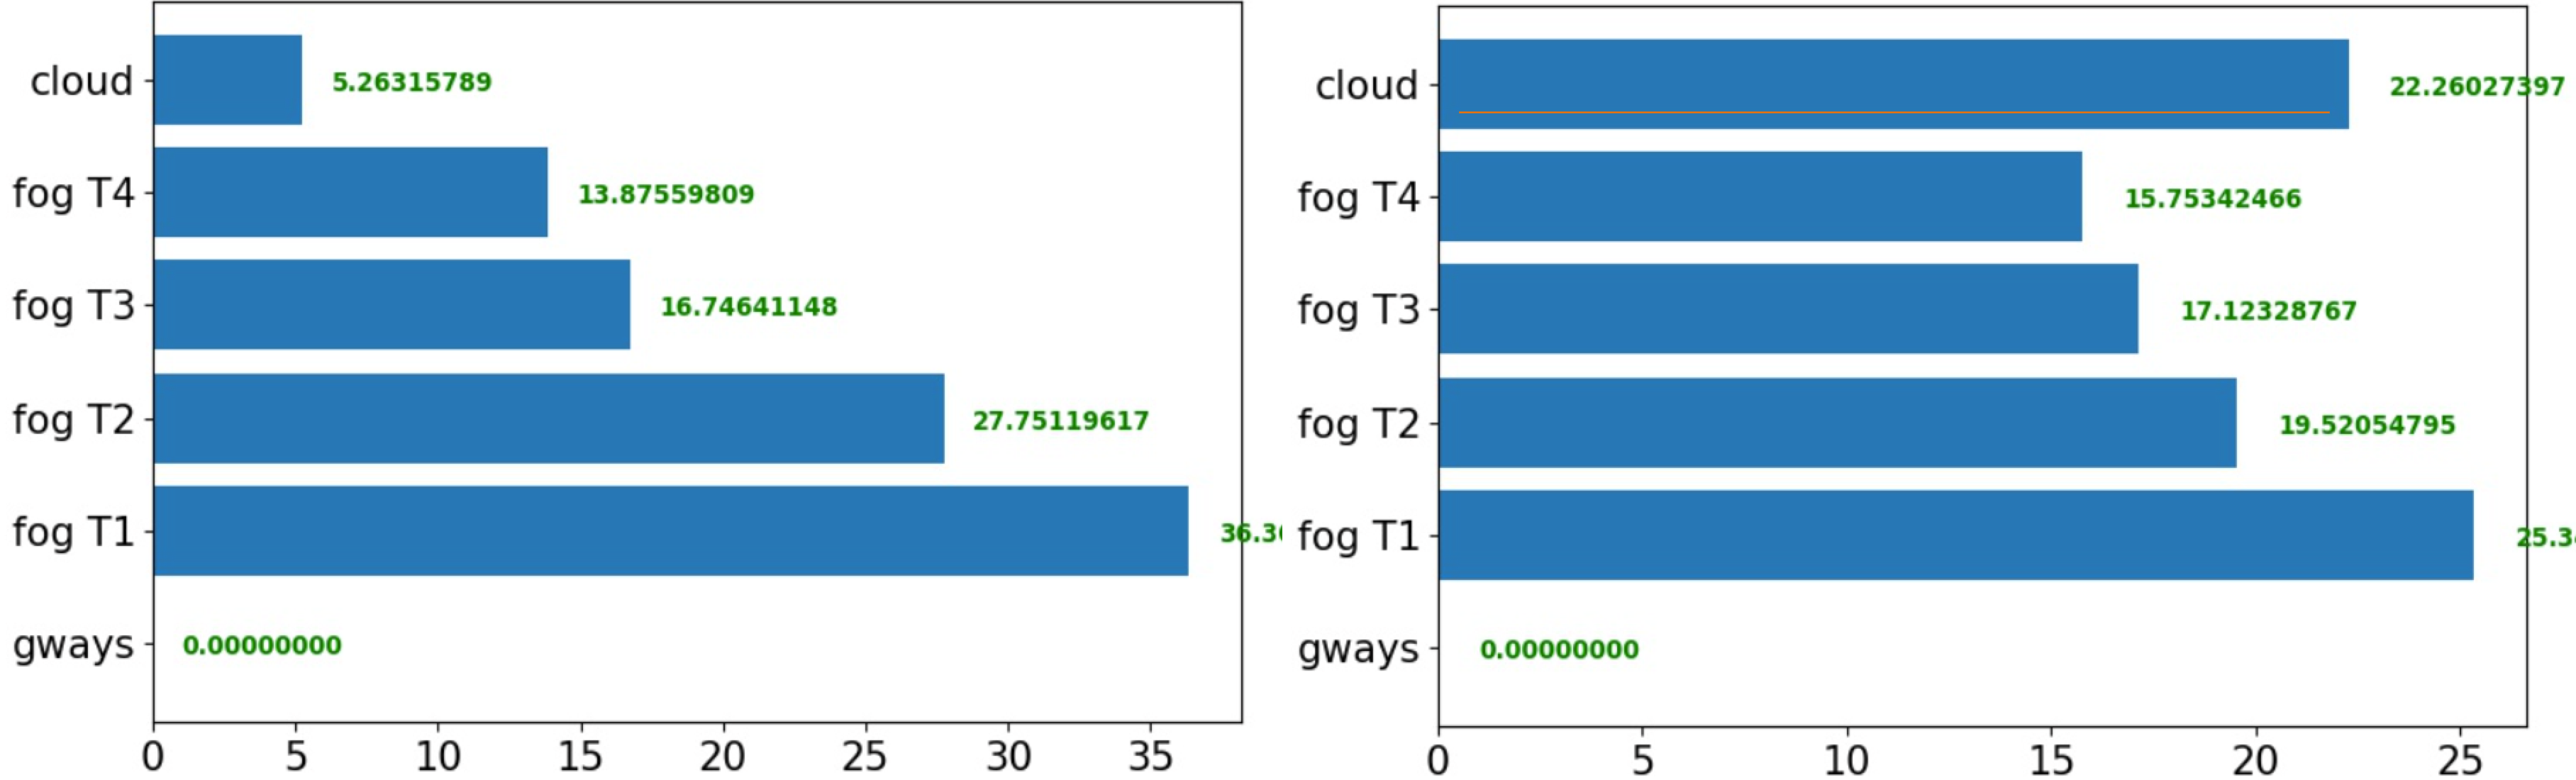
\includegraphics[width=14cm]{images/min_conn_to_upper_levels_comparison}
  \centering
  \caption{Percentuale di servizi correttamente allocati in ogni livello. A sinistra con \texttt{MIN\_CONN\_TO\_UPPER\_LEVELS = 20}, a destra con \texttt{MIN\_CONN\_TO\_UPPER\_LEVELS = 200} pari a 3.}
  \label{fig:min_conn_to_upper_levels_comparison}
\end{figure}

Per valutare il \textit{fault tollerance} della rete sono state eseguite due simulazioni e le rispettive analisi, valutando il soddisfacimento delle richieste prima nello scenario con \texttt{MIN\_CONN\_TO\_UPPER\_LEVELS = 10} e \texttt{MAX\_CONN\_TO\_UPPER\_LEVELS = 20} (Figura \ref{fig:min_conn_20_sim_2}) e poi nello scenario con \texttt{MIN\_CONN\_TO\_UPPER\_LEVELS = 200} e \texttt{MAX\_CONN\_TO\_UPPER\_LEVELS = 210} (Figura \ref{fig:min_conn_200_sim_1}).

\begin{figure}[!ht]
  \includegraphics[width=14cm]{images/min_conn_10_sim_2}
  \centering
  \caption{Numero di richieste soddisfatte durante la simulazione, con e senza failure control.}
  \label{fig:min_conn_20_sim_2}
\end{figure}

\begin{figure}[!ht]
  \includegraphics[width=14cm]{images/min_conn_200_sim_1}
  \centering
  \caption{Numero di richieste soddisfatte durante la simulazione, con e senza failure control.}
  \label{fig:min_conn_200_sim_1}
\end{figure}